% TEMPLATE for Usenix papers, specifically to meet requirements of
%  USENIX '05
% originally a template for producing IEEE-format articles using LaTeX.
%   written by Matthew Ward, CS Department, Worcester Polytechnic Institute.
% adapted by David Beazley for his excellent SWIG paper in Proceedings,
%   Tcl 96
% turned into a smartass generic template by De Clarke, with thanks to
%   both the above pioneers
% use at your own risk.  Complaints to /dev/null.
% make it two column with no page numbering, default is 10 point

% Munged by Fred Douglis <douglis@research.att.com> 10/97 to separate
% the .sty file from the LaTeX source template, so that people can
% more easily include the .sty file into an existing document.  Also
% changed to more closely follow the style guidelines as represented
% by the Word sample file. 
% This version uses the latex2e styles, not the very ancient 2.09 stuff.
\documentclass[letterpaper,twocolumn,10pt]{article}
\usepackage{usenix,epsfig,endnotes,url}
\begin{document}

%don't want date printed
\date{}

%make title bold and 14 pt font (Latex default is non-bold, 16 pt)
\title{  Chukwa: A large-scale monitoring system}

%for single author (just remove % characters)
\author{
{\rm Jerome Boulon}\\
{\rm jboulon@yahoo-inc.com}\\
Yahoo!, inc
\and
{\rm Andy Konwinski}\\
{\rm andyk@cs.berkeley.edu}\\
UC Berkeley
\and
{\rm Runping Qi}\\
{\rm runping@yahoo-inc.com}\\
Yahoo!, inc
\and
{\rm Ariel Rabkin}\\
{\rm asrabkin@cs.berkeley.edu}\\
UC Berkeley
\and
{\rm Eric Yang}\\
{\rm eyang@yahoo-inc.com}\\
Yahoo!, inc
\and
{\rm Mac Yang}\\
{\rm macyang@yahoo-inc.com}\\
Yahoo!, inc
% copy the following lines to add more authors
% \and
% {\rm Name}\\
%Name Institution
} % end author

\maketitle

% Use the following at camera-ready time to suppress page numbers.
% Comment it out when you first submit the paper for review.
%\thispagestyle{empty}

\begin{abstract}

We describe the design and initial implementation of Chukwa, a data collection system for monitoring and analyzing large distributed systems. Chukwa is built on top of Hadoop, an open source distributed filesystem and MapReduce implementation, and inherits Hadoop's scalability and robustness. 
%Chukwa demonstrates that a distributed filesystem and MapReduce implementation are general distributed computing primitives, that can be utilized effectively in 
Chukwa also includes a flexible and powerful toolkit for displaying monitoring and analysis results, in order to make the best use of this collected data. 

\end{abstract}

\section{Introduction}
\label{sec:introduction}

Hadoop is a distributed filesystem and MapReduce \cite{mapreduce} implementation that is used pervasively at Yahoo! for a variety of critical business purposes.  Production clusters often include thousands of nodes. Large distributed systems such as Hadoop are fearsomely complex, and can fail in complicated and subtle ways. As a result, Hadoop is extensively instrumented.  A two-thousand node cluster configured for normal operation generates nearly half a terabyte of monitoring data per day, mostly application-level log files.

%I think we need to state that this is not intended only for Hadoop related data, but for all applications that run on our cluster, with Hadoop as the first customer, with others following closely on Hadoop's heels (who else do we have lined up here?)
This data is invaluable for debugging, performance measurement, and operational monitoring.  However, processing this data in real time at scale is a formidable challenge. A good monitoring system ought to scale out to very large deployments, and ought to handle crashes gracefully.  In Hadoop, only a handful of aggregate metrics, such as task completion rate and available disk space, are computed in real time. The vast bulk of the generated data is stored locally, and accessible via a per-node web interface.  Unfortunately, this mechanism does not facilitate programmatic analysis of the log data, nor the long term archiving of such data.

To make full use of log data, users must first write ad-hoc log aggregation scripts to centralize the required data, and then build mechanisms to analyze the collected data.  Logs are periodically deleted, unless users take the initiative in storing them.
% [?cite matei @ facebook who did exactly this for them?]

We believe that our situation is typical, and that local storage of logging data is a common model for very large deployments.  To the extent that more sophisticated data management techniques are utilized, they are largely supported by ad-hoc proprietary solutions.  
A well documented open source toolset for handling monitoring data thus solves a significant practical problem and provides a valuable reference point for future development in this area. 

We did not aim to solve the problem of real-time monitoring for failure detection, which systems such as Ganglia already do well. Rather, we wanted a system that would process large volumes of data, in a timescale of minutes, not seconds, to detect more subtle conditions, and to aid in failure diagnosis. Human engineers do not generally react on a timescale of seconds, and so a processing delay of a few minutes is not a concern for us.

Such a data collection system ought not be developed in isolation. Many problems inherent in monitoring can be solved by relying on existing scalable distributed computing platforms. In particular, we believe that a distributed filesystem is a natural tool for data storage, and that MapReduce is a natural way of processing monitoring data. Leveraging this existing infrastructure drastically reduces the engineering difficulty inherent in large-scale monitoring.
 
 We are in the process of building a system, which we call Chukwa, to demonstrate that practical large-scale can be readily built atop this existing infrastructure. \footnote{In Hindu mythology, Chukwa is the turtle that holds up Maha-pudma, the elephant that hold up the world.  This name is especially appropriate for us, since the the Hadoop mascot is a yellow elephant.}   
 it uses Hadoop's distributed file system (HDFS) as its data store, and relies on MapReduce jobs to process the data. By leveraging these existing tools, Chukwa can scale to thousands of nodes in both collection and analysis capacities, while providing a standardized and familiar framework  for processing the collected data. Many components of Chukwa are pluggable, allowing easy customization and enhancement.
 
The core components of Chukwa are largely complete, and we expect the system to enter production use at Yahoo! within the next few months. We have some initial operational experience, and preliminary performance metrics.    We begin by discussing our goals and requirements in some detail.  We then describe our design, explaining our motivation for various decisions. We then present some performance data, and conclude by offering some comparisons with related work.

\section{Goals and requirements} 


There are two key figures of merit for monitoring systems such as Chukwa: scale and latency.  We intend to use Chukwa to monitor multiple clusters of several thousand hosts, potentially generating several terabytes of data per day.  Our initial goal was a latency of less than ten minutes between the generation of data on cluster nodes and its availability in HDFS for centralized analysis using Hadoop MapReduce. We believe that our design can operate effectively with latencies closer to a minute, as discussed in our conclusion.  Few useful actions can be taken on timescales significantly shorter than that, and therefore we do not believe this limit will be problematic for us.%this statement may need more support

The initial goal for Chukwa is to monitor and analyze several-thousand-node Hadoop deployments. Nothing in our design restricts us from monitoring other clusters, however our goals are primarily driven by the motivating example of Hadoop.  Analysis encompasses many goals:  
\begin{itemize}
\item
Providing canned reports to meet known needs for accounting, capacity planning, performance characterization, utilization.  Some examples:
%\begin{itemize}
%\item 
%Summarize grid usage: disk usage / CPU total, grouped by account, project, and user.  
%\item 
%  Measure performance improvement across Hadoop versions
%  \item 
%  Assess the quality of service based on waiting time, node availability, and service uptime
%\end{itemize}
These can be done in a straightfoward way via MapReduce jobs, provided that the data has been stored suitably.  
\item
 Reducing the number and extent of outages through trend analysis and anomaly detection to identify at-risk elements such as compute nodes, name node, switches 
\item
  Contributing to Hadoop development in robustness and performance by making possible the analysis of jobs and infrastructure along many different dimensions
\item
   Reducing the number of false alerts and increasing the value and confidence level of true alerts through correlation of metrics and environmental information
\item
    Reducing the time and effort required to identify and resolve cluster issues by highlighting trouble spots and by correlating metrics and environmental information to provide the required context and history, as well as by bringing together all required tools in one place.
\end{itemize}

Chukwa can collect a large and open-ended set of time series metrics and logs, as well as  slowly changing dimensions such as machine configuration, related to the state, behavior, characterization, and performance of a Hadoop cluster and processes running on it. Stored data will be available indefinitely, limited only by storage capacity, and not by retrieval speed.  

%Chukwa should be robust against agent crashes

\section{Data Collection}

\begin{figure}
 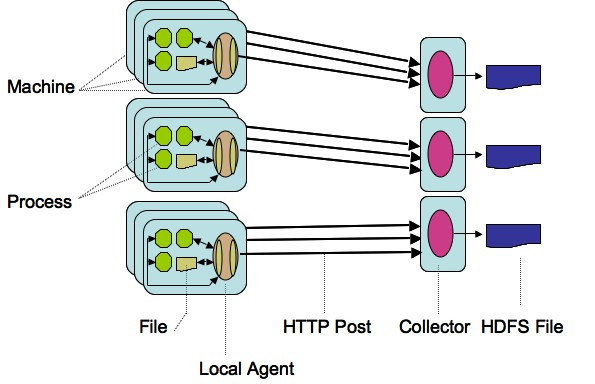
\includegraphics[width=75mm]{chukwa0.jpg}
\caption{The Chukwa collection architecture} 
\end{figure}

\begin{figure}
  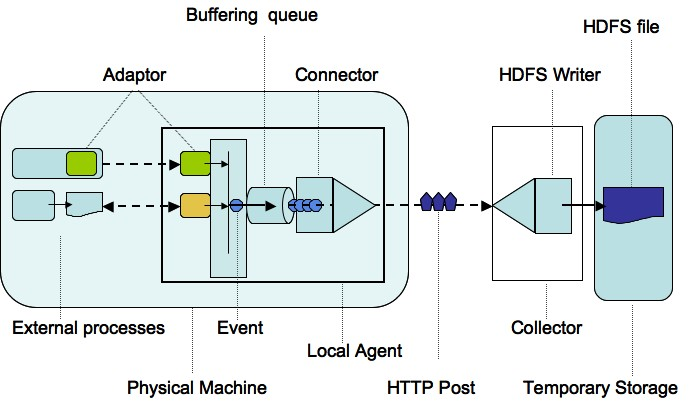
\includegraphics[width=75mm]{chukwa1.jpg}
\caption{The agent side}
\end{figure}

To achieve our scalability goals, we opted early in the design process to make HDFS our chief storage technology. HDFS installations can store petabytes of data, and support fairly high throughput. HDFS also facilitates parallel processing of stored data with MapReduce.

Chukwa thus breaks into two halves -- the pipeline for getting data into a convenient format in HDFS, and a toolkit for analyzing data using MapReduce and displaying it in a helpful way. A pipelined approach to data collection aids flexibility, by providing natural points for adding functionality. We discuss each section of the pipeline in turn, before discussing the user interface and analysis tools offered by Chukwa.

\subsection{Adaptors}

The particular data being collected about a machine will change with time, and from machine to machine. As Hadoop tasks start and stop, different log files must be monitored. We might want to increase our collection rate if we detect anomalies.  And of course, the monitoring package on a given machine must be customized according to the services running on that machine: it makes no sense to collect Hadoop metrics on an NFS server.

As a result, we bundle data collection into small dynamically loadable Adaptors.  At present, Chukwa includes adaptors to collect Hadoop logs, application metrics, and system telemetry. We expect to write adaptors for tasks like counting recoverable disk read errors, retrieving causal logs from X-Trace \cite{xtrace}, and monitoring operating system and Java virtual machine state. 

%FIXME: ruby/failmon
%The output of an adaptor consists of chunks, each containing one or more semantically meaningful records.  These records, such as lines from a log file or batches of metrics, must be kept together.  This means that adaptors must parse files intensively enough to detect record boundaries, and they must correctly handle buffering.

%These costs are offset by important advantages. Keeping records intact allows collectors to run filters or triggers against data streams, without having to buffer partial lines. In the presence of load balancing across collectors, these filters will still behave properly. Perhaps most importantly, this allows the map phase of the periodic MapReduce process to extract metadata from records and use this metadata as a sort key: a large performance win.  If records were split across collectors, this metadata could be inaccessible.

%FIXME: say something here
%After a crash, the local agent restarts each adaptor, passing sequence number of the last byte of their output that was successfully sent to a collector.  Adaptors that read from files can seek to that offset before starting.  Adaptors that output ephemeral data, such as CPU load, can simply begin numbering output from this point, to mask  any crash-induced discontinuity from downstream users. 

\subsection{Agent}

Adaptors run within a local agent process on each machine. This process is left permanently running, and is restarted automatically if it crashes. The agent process is responsible for starting and stopping adaptors in response to external commands.  It also provides two crucial services to adaptors. First, it is responsible for forwarding chunks over HTTP to the collectors, where they are written to stable storage. Second, it is responsible for making regular checkpoints of adaptor state, and restarting adaptors at the appropriate position after a crash.  This checkpoint mechanism ensures that data is appropriately resent after a crash.

We opted to put most of the recovery logic in the agents, rather than the collectors. This removes state from the collectors. We considered having agents check with collectors to find out what the last thing they sent was. However, each agent would have to check with each collector, resulting in an exorbitant number of connections if many agents fail and reboot simultaneously.

\subsection{Collector}

The collector is a web service (implemented as a Java servlet) that receives chunks via HTTP, and writes them to stable storage in the Hadoop distributed file system.  

Each collector writes to a sink files in the Hadoop distributed file system. Each sink file contains a sequence of chunks, potentially from many different streams.  Every few minutes, collectors ``rotate'' sink files, by closing their current sink files, and marking them as available for processing. While it would make sense to use HDFS files as circular buffers, the filesystem semantics forbid this.  Instead, each collector closes its current sink file every few minutes, and marks it available for processing.  

An alternate design would be to have each local agent dump its results directly into HDFS. Unfortunately, HDFS does not perform well for filesystems with large numbers of files, due to contention and space limits at the Namenode.  The many-to-one relationship between hosts and collectors helps significantly, although if Chukwa deployments got big enough, some more drastic step might be needed.

Another advantage of having collectors is that it allows us to hide the details of the Chukwa storage cluster, such as its Hadoop version from the agents.  This is important, for instance, when using Chukwa to monitor a development cluster running an unstable version of Hadoop or when using Chukwa to monitor a non-Hadoop cluster.  

\subsection{Demux and archiving}

A pair of MapReduce jobs run every few minutes, taking these sink files as input.  The first job simply archives all the collected data, without processing or interpreting it.  The second job parses out structured data from some of the logs, and loads this structured data into a data store.   For performance reasons, we do record parsing in the Map phase, and extract key-value pairs. Example records include job history reports, task durations, and so forth. We then use the shuffle and sort phases of the Reduce to organize records semantically by application timestamp and type. This forced us to design our adaptors to have adaptors output meaningful records, and not arbitrary chunks of streams. %% FIXME: recast last sentence

 These datastores are also pluggable. For now, we use HDFS files, one file per cluster, per data type, and time period.  So for instance there would be one file for all of a particular clusters datanode logs, for the period from noon to 1pm on a given day.   This is only an interim solution, and we are evaluating various more suitable data stores, with support for structured queries.  Hive, an HDFS-backed data warehouse might also be a good fit here. \cite{hive} 
 % Hive supports a subset of SQL for queries, which is particularly appealing for the context of ad-hoc analytics. 
 Column-oriented databases such as HBase, and Hypertable would also be sensible options.  For small deployments, a local relational database would be suitable.

%This de-multiplexing is the phase of Chukwa processing with the highest latency. Hadoop TaskTrackers only poll for work every few seconds, and therefore map-reduce jobs have an inherent latency larger than that.  Unfortunately, we do need this de-multiplexing stage, since HDFS, and structured stores built on top of it, perform much better for large writes than for small ones.

Data stored in HDFS in a structured format can be processed straightforwardly with MapReduce jobs. We envision a library of ``canned'' MapReduce jobs for tasks like finding common failure modes, correlating events in the logs with slowdowns, discovering flakey machines, and so forth.  Since Chukwa data is split into different files based on content, these jobs take as input only a small fraction of the total data volume, and therefore can run relatively quickly.  Most structured storage systems, including Hive and Hypertable, include their own query interfaces. We expect that these interfaces will be used by users who want to do simple ad-hoc queries over stored Chukwa data, with MapReduce being reserved for more complex processing.


\section{Data Analysis and Display}



Collected data is only as useful as the analysis that can be done on it.  To ease analysis of collected data, we've built a flexible, configurable, ``portal-style'' web interface to Chukwa, termed the Hadoop Infrastructure Care Center (HICC). A configurable interface is not simply a frill --- it is necessary, since different users have very different data analysis needs.

\begin{figure}
% 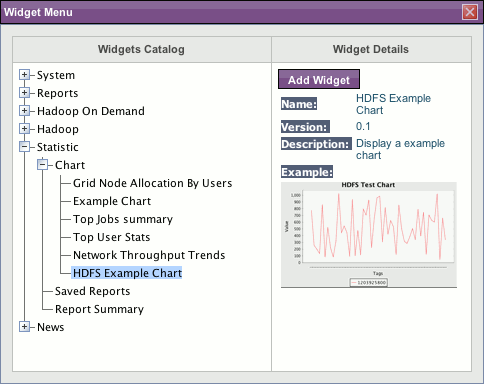
\includegraphics[width=75mm]{widget.png}
%\caption{The HICC widget catalog} 
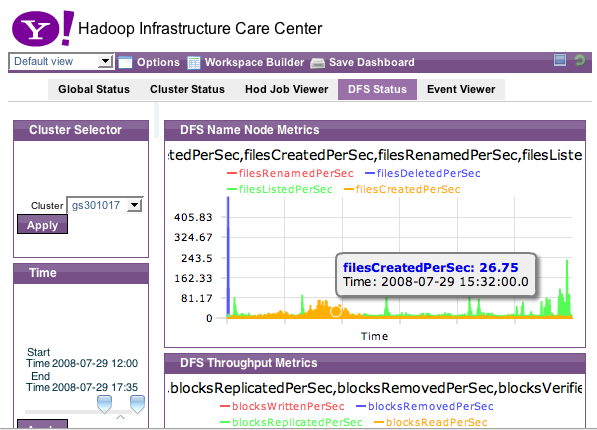
\includegraphics[width=75mm]{hicc_in_action2.png}
\caption{HICC displaying some DataNode metrics}
\end{figure}

\subsection{The Use Model}

We expect HICC to be used by four different (though overlapping) constituencies:   users, operators, managers, and developers.  These different groups have different characteristic questions:


\begin{itemize}
\item Users will ask how far along their jobs are, and what resources are available for future jobs. They need access to the logs and output from their jobs.  

\item Operators need to be notified of hardware failures and performance anomalies. They need to be warned about resource shortages, such as storage exhaustion.  

\item Managers need guidance in provisioning, and in apportioning costs. This means that they need tools for analyzing past usage by users and groups, and for projecting future demands.   They need access to figures of merit, such as average job waiting time.

\item Developers need information about the performance in operation, bottlenecks within Hadoop, common failure patterns, and so forth.

\end{itemize}

\subsection{How HICC works}

In practice, a single individual often fulfills more than one of these roles, or some portion of a role. As a result, there is a compelling need to allow individuals to mix and match different components. We chose to do this by bundling each query, or family of queries, into a widget. HICC users can assemble their HICC workspace by selecting widgets from a catalog, in exactly the way that they can customize their personal Yahoo! or Google portal pages.

Some of these components will display the results of canned map-reduce jobs run against data in  Chukwa storage.  Others will perform on-the-fly queries against SQL databases.    Still others might display telemetry collected with Ganglia, or report on recently opened failure tickets.  

HICC stores several kinds of widget state.  There is a global context, through which different widgets can ``collaborate'' and share data. There is a dashboard view, which stores information about the user's preferred layout, and display settings.  There is a widget descriptor file, for storing widget configuration and parameters.   

%HICC is not intended for exploratory, ad-hoc queries. For that, we expect to rely on the query interface of our structured data store.  Since this store is not yet available, we have been using a MySQL database.

\section{Evaluation}

%Chukwa is currently in development, and we have not yet been able to do large-scale tests.  However, we have reason to be confident that Chukwa will comfortably meet our performance goals.

Using logs from a production cluster at Yahoo!, we found that a 2000-node production cluster would generate around 5.5 MB of data per second.  Of this, the vast bulk (more than 95\%) was task tracker logs.  Metrics data accounted for more than half the remainder, with Namenode, HDFS datanode, and JobTracker logs accounting for the rest. This data rate is small enough that Chukwa should impose only very modest overhead on datacenter networks. 

  We conducted a number of small experiments to verify that Chukwa could handle this sort of load.   All tests were run on an internal development cluster at Yahoo.  Machines had four 2.8 GHz Xeon processors, four IDE disks, and 3 GB of RAM, and ran Linux, with a 2.6.9 kernel.  %kernel version 2.6.9-55

We checked for performance limitations at three places: the collector, the HDFS cluster and the map-reduce job.
To assess collector throughput, we disabled HDFS writes, and measured the throughput between a single agent and collector, connected by gigabit ethernet.  We found that throughput was around 80 MB/sec, and that this limit was imposed by network latency.  Handling this input took only half of one CPU on the collector side, which is an affordable overhead. 

A single Chukwa collector was easily able to saturate the HDFS back-end with very modest CPU cost. Our five-node HDFS test cluster saturated at about 25 megabytes per second.  Even writing 25 megabytes per second, the collector was only using about 10\% of a single core. This is an encouraging number, since it suggests that even small monitoring clusters have ample write bandwidth for current as well as future data collection demands.  

%The bottleneck in our current design is the demux job.  As mentioned, limitations in Hadoop restrict performance 
%we expect that our write bandwidth would increase if we added additional collectors, since using more than one writer enables the HDFS datanodes to concurrently write across multiple physical disks.  

As mentioned, the bottleneck in our design is the Demux job. We found that our Demux job can easily keep up with incoming data.  Using four worker nodes, we were able to process a gigabyte of data in two and a half minutes; for a throughput of 6.6 MB/sec, which exceeds our target data rate. Larger data volumes improved efficiency significantly:  with 2 GB of data, the processing rate went up to 8.5 MB/sec. Optimizing MapReduce jobs is a reasonably well understood science, and we believe that significant gains can be readily achieved here. 

These results show that Chukwa can maintain latencies well under our ten minute target, while imposing very modest overheads on the cluster: five Chukwa nodes are only 0.25\% of our notional 2000-node cluster. We expect to be able to maintain these latency targets as we scale up the number of nodes being monitored.  Ramping up the size of MapReduce jobs is routine, and the engineering issues are well understood. Even for monitoring hundreds of thousands of nodes, Chukwa's data volumes would be significantly smaller than those seen in our production web indexing clusters.


\section{Related Work}
%\label{sec:related}

Chukwa represents a design point in between two existing classes of systems: log collection frameworks on the one hand, and network management systems on the other.  Chukwa intends to combine the abundance of data display tools of existing NMS systems, with the high throughput and robustness expected of log collection frameworks.

The syslog protocol supported streaming logs across the network as long ago as the late 1980s.  However, syslog had serious defects: no clear solution to the discovery, load balancing, or failure handing problems.  The Scribe system apparently solves some of these problems, but unfortunately, no details of scribe have been published.

Chukwa has some similarity with network monitoring systems such as Nagios, Ganglia, or Tivoli Monitoring \cite{Ganglia, Nagios, tivmon}. The three systems differ in emphasis, but have important commonalities.  All are capable of collecting and storing substantial volumes of metrics data. All include tools for displaying this data.  Nagios and Tivoli monitoring have centralized architectures, while Ganglia is decentralized.  Ganglia, unfortunately, is heavily adapted towards numeric time-series data, and provides minimal support for the sort of complex text-processing necessary for our applications.

\section{Conclusion}
%\label{sec:conclusion}

Chukwa provides a flexible and powerful toolkit for analyzing displaying collected data.  We expect Chukwa to be very useful in monitoring and managing large system deployments.

Building Chukwa on top of Hadoop resulted in a few design quirks, and a modest latency penalty.  However, it greatly simplified implementation, and leverages the substantial amount of work going into Hadoop.  Hadoop 0.19, which will be released within a few months, should significantly improve the performance of short-running Map tasks, which will allow us to efficiently operate Chukwa on short timescales.

%\iffalse
%\subsection{Future Work}
%\fi

%\section{Acknowledgments}

\addcontentsline{toc}{section}{References}
\begin{thebibliography}{99}

\bibitem{mapreduce}
Jeffrey Dean and Sanjay Ghemawat. ``MapReduce: Simplified Data Processing on Large Clusters.'' \newblock In \textit{Communications of the ACM}, Volume 51, Issue 1, pp. 107-113, 2008.
\bibitem{Ganglia}
Matthew L. Massie, Brent N. Chun, and David E. Culler.  ``The Ganglia Distributed Monitoring System: Design, Implementation, and Experience''.
\newblock In \textit{Parallel Computing} Volume 30, Issue 7, pp 817-840, 2004.
\bibitem{Nagios}
http://www.nagios.org/
\bibitem{tivmon}
IBM Tivoli Monitoring.
\newblock Available online: \texttt{http://www.ibm.com/ software/ tivoli/ products/ monitor/}
\bibitem{hive}
Joydeep Sen Sarma.  ``Hive as a contrib project''
\newblock Available online: https://issues.apache.org/jira/browse/HADOOP-3601
\bibitem{xtrace}
Rodrigo Fonseca, George Porter, Randy H. Katz, Scott Shenker, and Ion Stoica.  X-Trace: A Pervasive Network Tracing Framework.
\newblock In \textit{4th USENIX Symposium on Networked Systems Design \& Implementation (NSDI'07)}, Cambridge, MA, USA, April 2007.
\end{thebibliography}

\end{document}

%		TODO:
%	Maybe more depth in related work
%	More performance numbers
%	Mention "work in progress" somewhere up front?
%	Better screen shot for HICC



